\chapter{Appendix}
\begin{landscape}
% i7 !!
\begin{figure}[H]
    \subfloat[Insertion time] {
        \includegraphics[width=1.0\textwidth]{plots/i7/plot_0_ts_sorted_bucketinsert}
    }
    \subfloat[Search] {
        \includegraphics[width=1.0\textwidth]{plots/i7/plot_0_ts_sorted_bucketsearch}
    }
    \label{fig:ts_i7_30m_sorted}
    \caption{Multithreaded scaling of the sorted dynamic array bucket with varying sizes on the
    i7 machine (4 cores). Testing done with the 30M dataset.}
\end{figure}
\begin{figure}[H]
    \subfloat[Insertion time] {
        \includegraphics[width=1.0\textwidth]{plots/i7/plot_0_ts_unsorted_bucketinsert}
    }
    \subfloat[Search] {
        \includegraphics[width=1.0\textwidth]{plots/i7/plot_0_ts_unsorted_bucketsearch}
    }
    \label{fig:ts_i7_30m_unsorted}
    \caption{Multithreaded scaling of the unsorted dynamic array bucket with varying sizes on the
    i7 machine (4 cores). Testing done with the 30M dataset. Note that the smaller bucket size tests did not complete. This is caused by lack of memory.}
\end{figure}
\begin{figure}[H]
    \subfloat[Insertion time] {
        \includegraphics[width=1.0\textwidth]{plots/i7/plot_0_ts_map_bucketinsert}
    }
    \subfloat[Search] {
        \includegraphics[width=1.0\textwidth]{plots/i7/plot_0_ts_map_bucketsearch}
    }
    \label{fig:ts_i7_30m_map}
    \caption{Multithreaded scaling of the STL::Map bucket with varying sizes on the
    i7 machine (4 cores). Testing done with the 30M dataset.}
\end{figure}
\begin{figure}[H]
    \subfloat[Insertion time] {
        \includegraphics[width=1.0\textwidth]{plots/i7/plot_0_ts_btree_bucketinsert}
    }
    \subfloat[Search] {
        \includegraphics[width=1.0\textwidth]{plots/i7/plot_0_ts_btree_bucketsearch}
    }
    \label{fig:ts_i7_30m_btree}
    \caption{Multithreaded scaling of the binary tree bucket with varying sizes on the
    i7 machine (4 cores). Testing done with the 30M dataset.}
\end{figure}
% ask !!
\begin{figure}[H]
    \subfloat[Insertion time] {
        \includegraphics[width=1.0\textwidth]{plots/ask/plot_0_ts_sorted_bucketinsert}
    }
    \subfloat[Search] {
        \includegraphics[width=1.0\textwidth]{plots/ask/plot_0_ts_sorted_bucketsearch}
    }
    \label{fig:ts_ask_30m_sorted}
    \caption{Multithreaded scaling of the sorted dynamic array bucket with varying sizes on the
    ask machine (8 cores). Testing done with the 30M dataset.}
\end{figure}
\begin{figure}[H]
    \subfloat[Insertion time] {
        \includegraphics[width=1.0\textwidth]{plots/ask/plot_0_ts_unsorted_bucketinsert}
    }
    \subfloat[Search] {
        \includegraphics[width=1.0\textwidth]{plots/ask/plot_0_ts_unsorted_bucketsearch}
    }
    \label{fig:ts_ask_30m_unsorted}
    \caption{Multithreaded scaling of the unsorted dynamic array bucket with varying sizes on the
    ask machine (8 cores). Testing done with the 30M dataset.}
\end{figure}
\begin{figure}[H]
    \subfloat[Insertion time] {
        \includegraphics[width=1.0\textwidth]{plots/ask/plot_0_ts_map_bucketinsert}
    }
    \subfloat[Search] {
        \includegraphics[width=1.0\textwidth]{plots/ask/plot_0_ts_map_bucketsearch}
    }
    \label{fig:ts_ask_30m_map}
    \caption{Multithreaded scaling of the STL::Map bucket with varying sizes on the
    ask machine (8 cores). Testing done with the 30M dataset.}
\end{figure}
\begin{figure}[H]
    \subfloat[Insertion time] {
        \includegraphics[width=1.0\textwidth]{plots/ask/plot_0_ts_btree_bucketinsert}
    }
    \subfloat[Search] {
        \includegraphics[width=1.0\textwidth]{plots/ask/plot_0_ts_btree_bucketsearch}
    }
    \label{fig:ts_ask_30m_btree}
    \caption{Multithreaded scaling of the binary tree bucket with varying sizes on the
    ask machine (8 cores). Testing done with the 30M dataset.}
\end{figure}
% c2d !!
\begin{figure}[H]
    \subfloat[Insertion time] {
        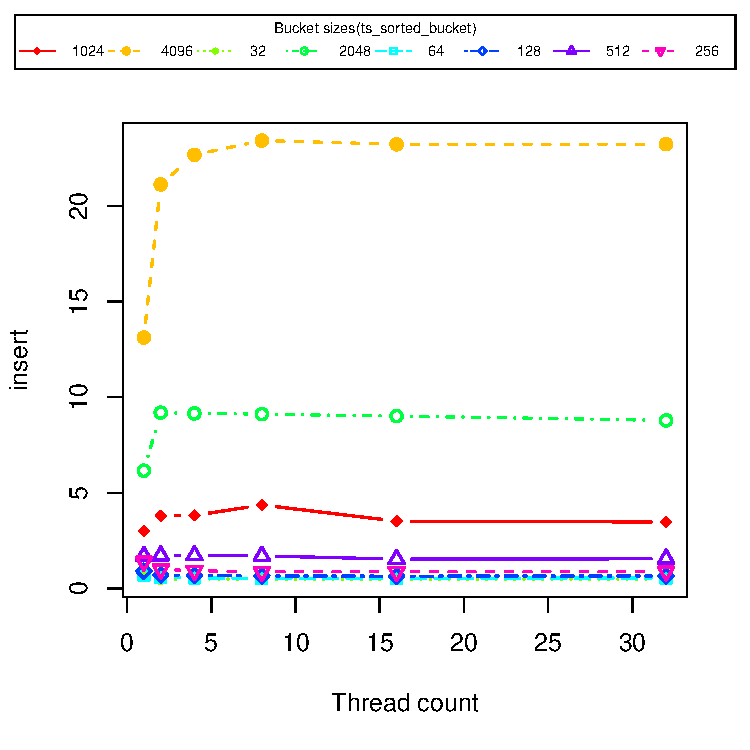
\includegraphics[width=1.0\textwidth]{plots/c2d/plot_1_ts_sorted_bucketinsert}
    }
    \subfloat[Search] {
        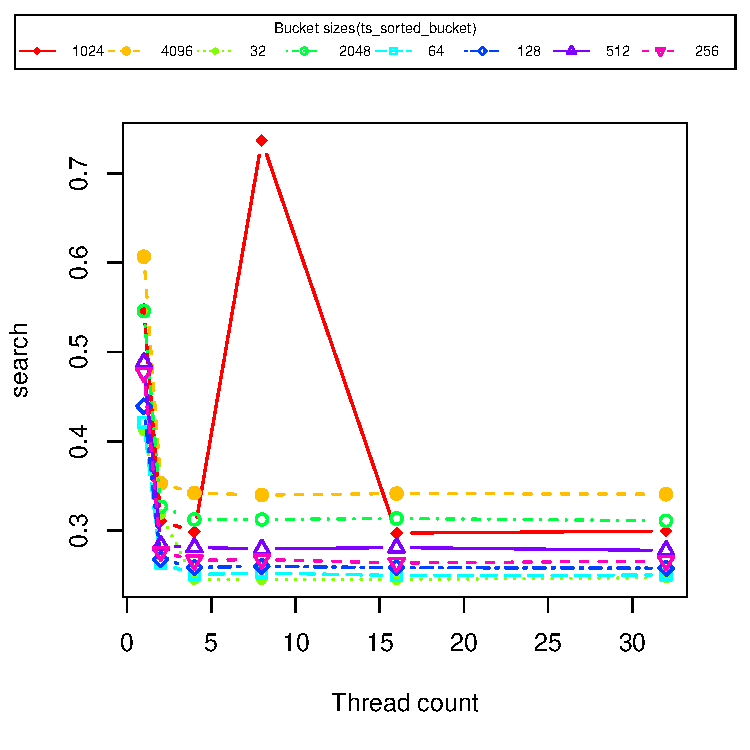
\includegraphics[width=1.0\textwidth]{plots/c2d/plot_1_ts_sorted_bucketsearch}
    }
    \label{fig:ts_c2d_shake_sorted}
    \caption{Multithreaded scaling of the sorted dynamic array bucket with varying sizes on the
    c2d machine (2 cores). Testing done with the shakespeare dataset.}
\end{figure}
\begin{figure}[H]
    \subfloat[Insertion time] {
        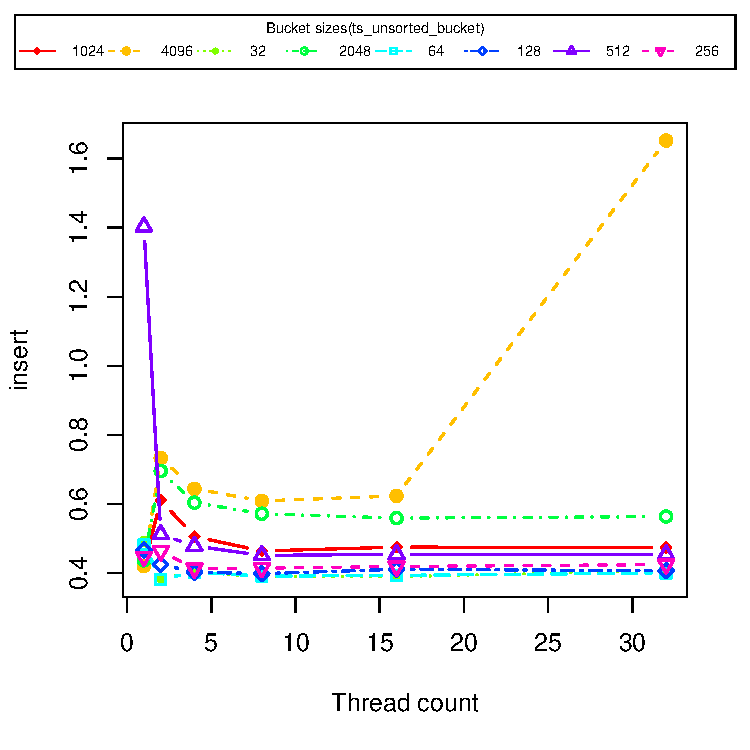
\includegraphics[width=1.0\textwidth]{plots/c2d/plot_1_ts_unsorted_bucketinsert}
    }
    \subfloat[Search] {
        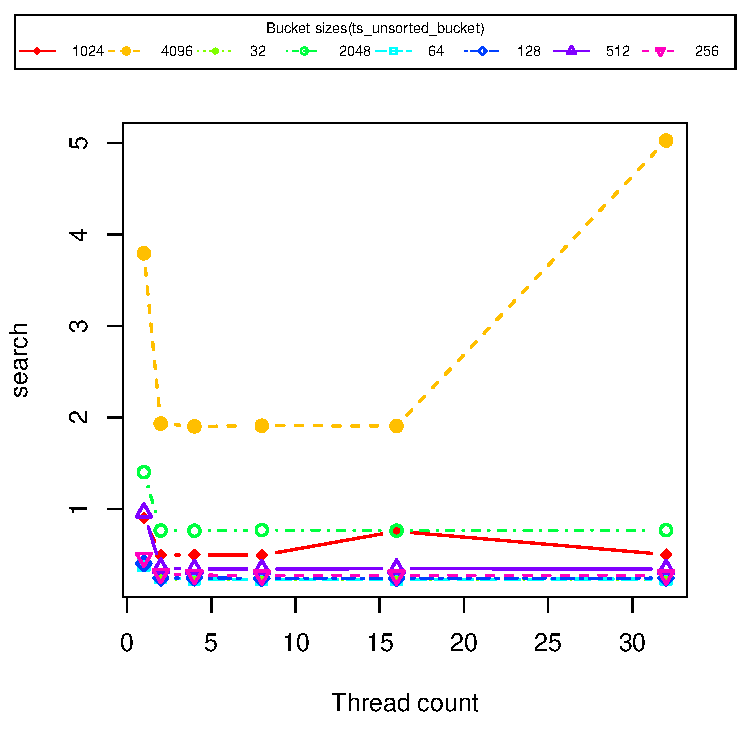
\includegraphics[width=1.0\textwidth]{plots/c2d/plot_1_ts_unsorted_bucketsearch}
    }
    \label{fig:ts_c2d_shake_unsorted}
    \caption{Multithreaded scaling of the unsorted dynamic array bucket with varying sizes on the
    c2d machine (2 cores). Testing done with the shakespeare dataset.}
\end{figure}
\begin{figure}[H]
    \subfloat[Insertion time] {
        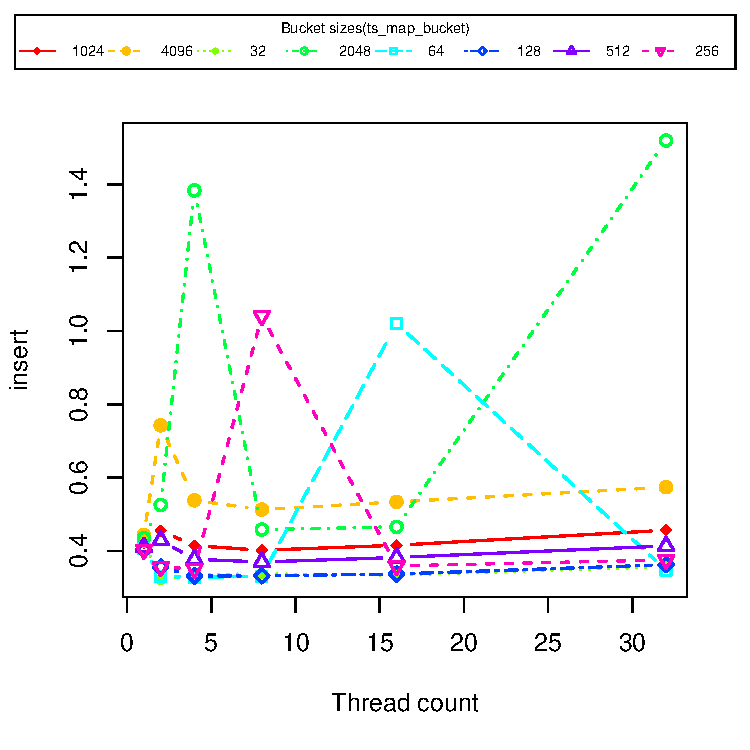
\includegraphics[width=1.0\textwidth]{plots/c2d/plot_1_ts_map_bucketinsert}
    }
    \subfloat[Search] {
        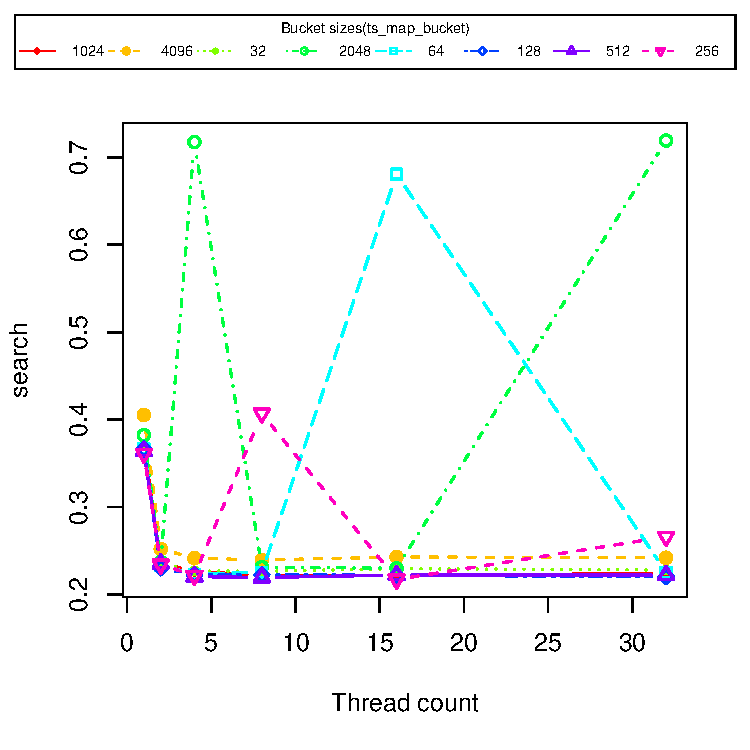
\includegraphics[width=1.0\textwidth]{plots/c2d/plot_1_ts_map_bucketsearch}
    }
    \label{fig:ts_c2d_shake_map}
    \caption{Multithreaded scaling of the STL::Map bucket with varying sizes on the
    c2d machine (2 cores). Testing done with the shakespeare dataset.}
\end{figure}
\begin{figure}[H]
    \subfloat[Insertion time] {
        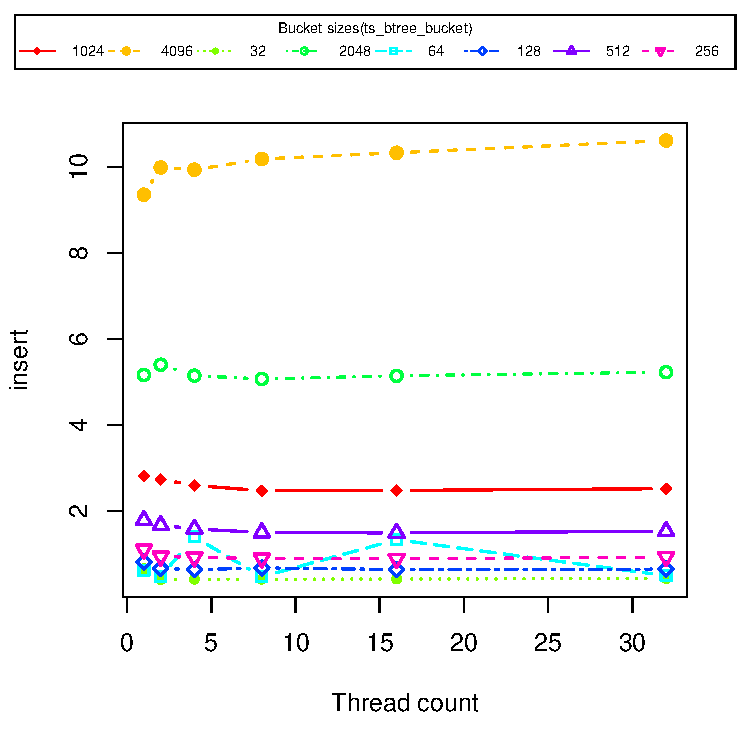
\includegraphics[width=1.0\textwidth]{plots/c2d/plot_1_ts_btree_bucketinsert}
    }
    \subfloat[Search] {
        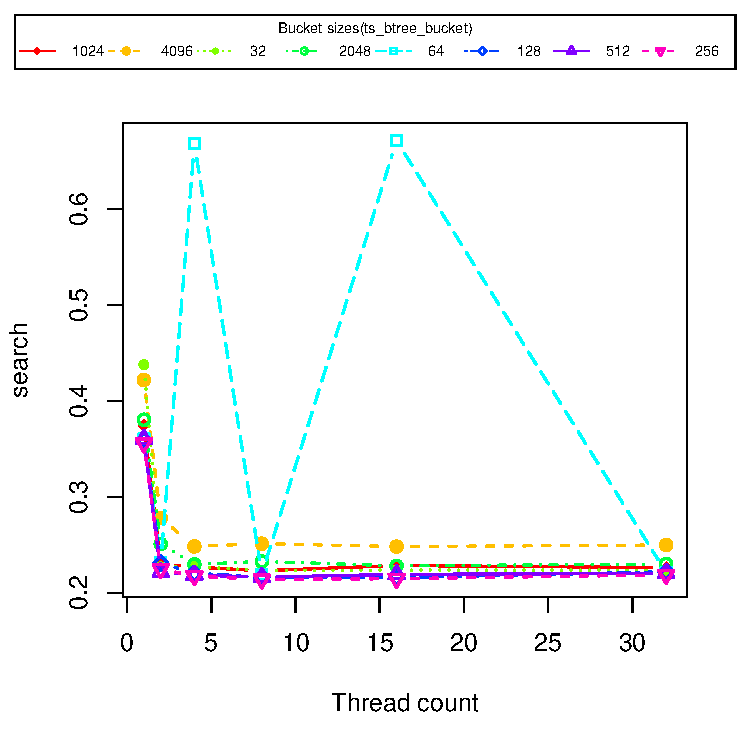
\includegraphics[width=1.0\textwidth]{plots/c2d/plot_1_ts_btree_bucketsearch}
    }
    \label{fig:ts_c2d_shake_btree}
    \caption{Multithreaded scaling of the binary tree bucket with varying sizes on the
    c2d machine (2 cores). Testing done with the shakespeare dataset.}
\end{figure}
% i7 !!
\begin{figure}[H]
    \subfloat[Insertion time] {
        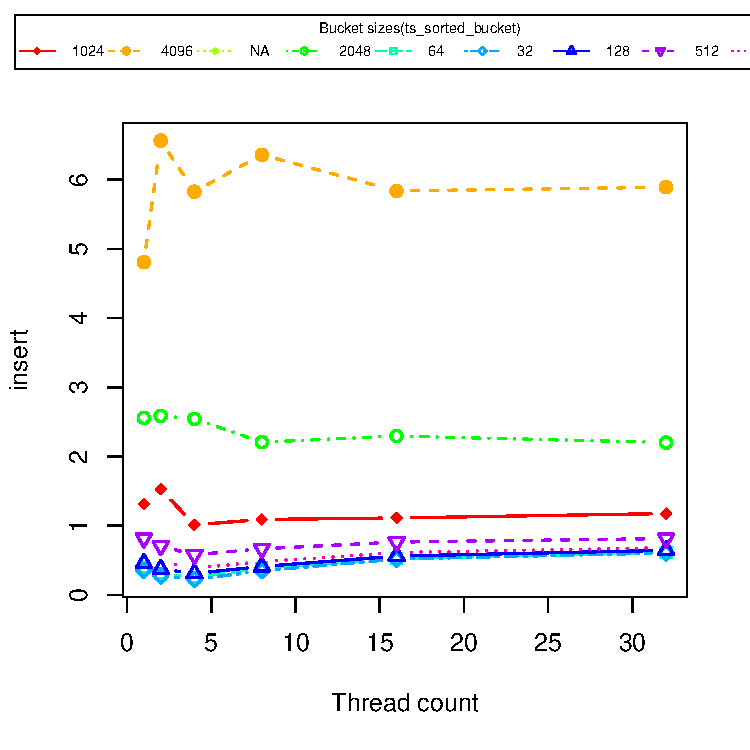
\includegraphics[width=1.0\textwidth]{plots/i7/plot_1_ts_sorted_bucketinsert}
    }
    \subfloat[Search] {
        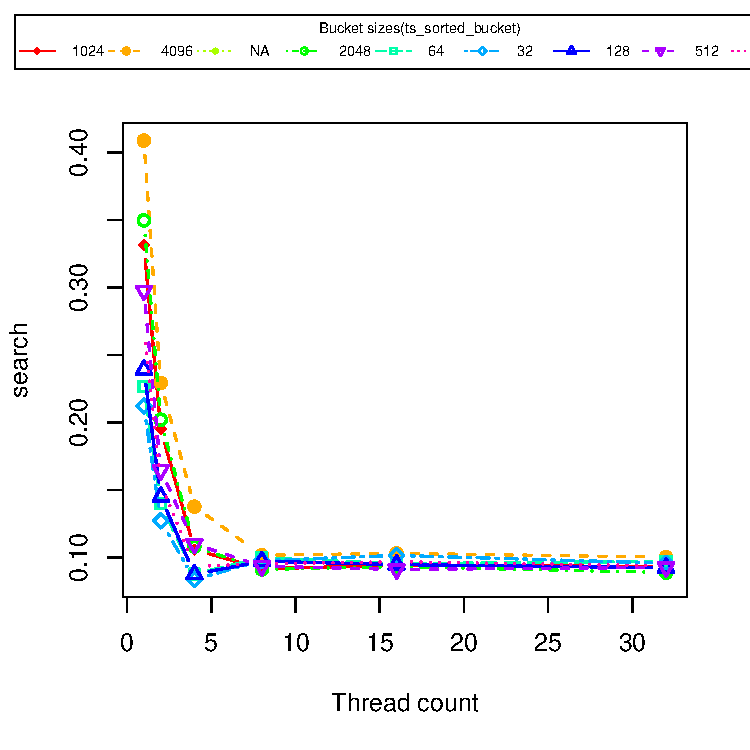
\includegraphics[width=1.0\textwidth]{plots/i7/plot_1_ts_sorted_bucketsearch}
    }
    \label{fig:ts_i7_shake_sorted}
    \caption{Multithreaded scaling of the sorted dynamic array bucket with varying sizes on the
    i7 machine (4 cores). Testing done with the shakespeare dataset.}
\end{figure}
\begin{figure}[H]
    \subfloat[Insertion time] {
        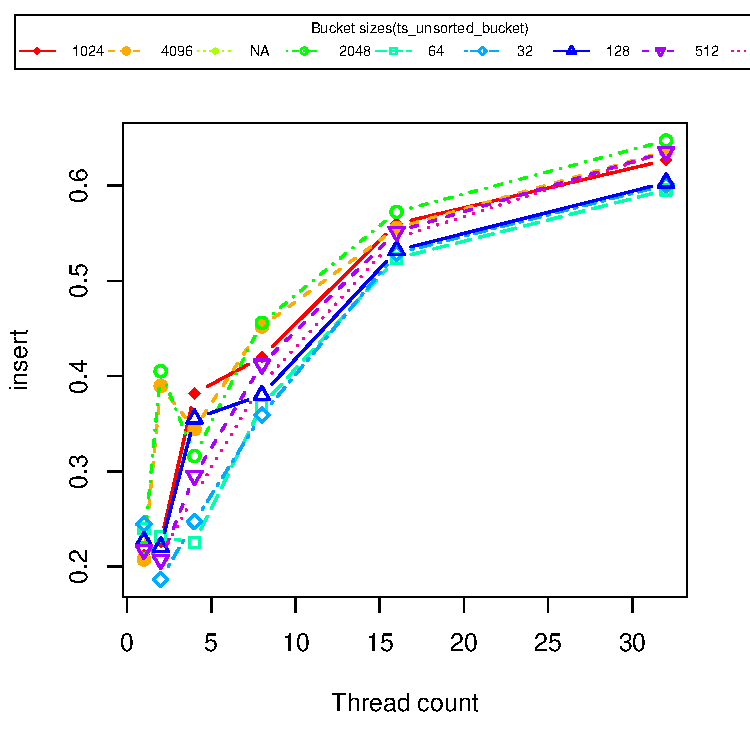
\includegraphics[width=1.0\textwidth]{plots/i7/plot_1_ts_unsorted_bucketinsert}
    }
    \subfloat[Search] {
        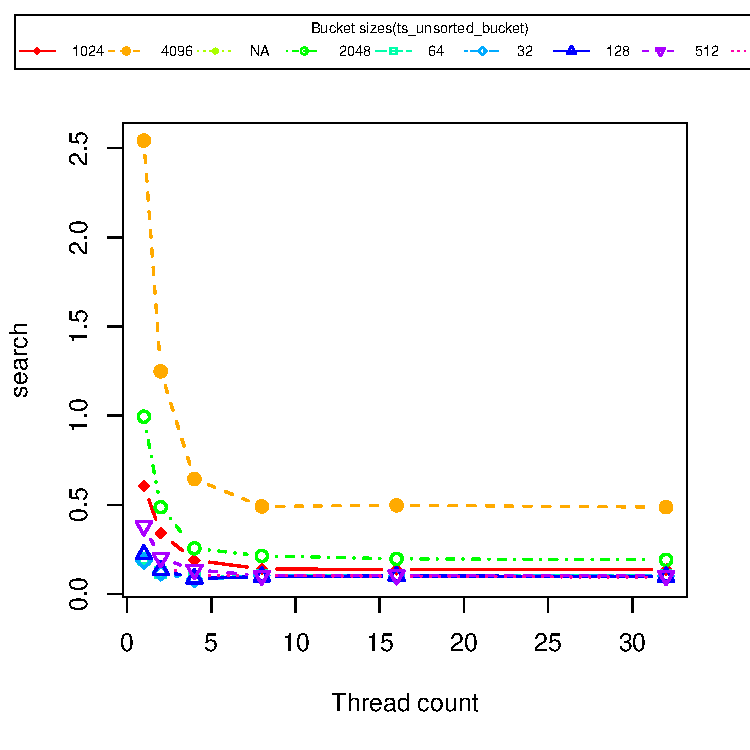
\includegraphics[width=1.0\textwidth]{plots/i7/plot_1_ts_unsorted_bucketsearch}
    }
    \label{fig:ts_i7_shake_unsorted}
    \caption{Multithreaded scaling of the unsorted dynamic array bucket with varying sizes on the
    i7 machine (4 cores). Testing done with the shakespeare dataset.}
\end{figure}
\begin{figure}[H]
    \subfloat[Insertion time] {
        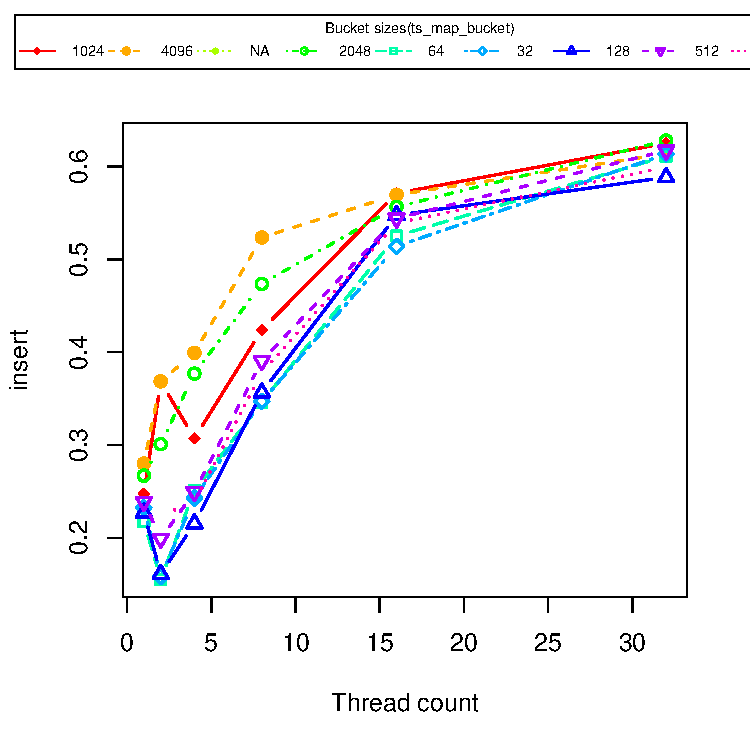
\includegraphics[width=1.0\textwidth]{plots/i7/plot_1_ts_map_bucketinsert}
    }
    \subfloat[Search] {
        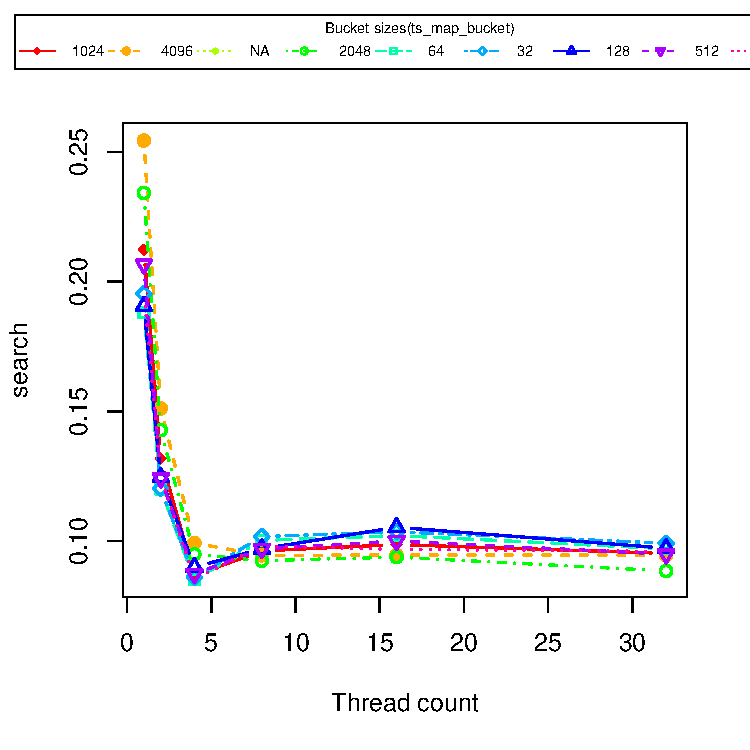
\includegraphics[width=1.0\textwidth]{plots/i7/plot_1_ts_map_bucketsearch}
    }
    \label{fig:ts_i7_shake_map}
    \caption{Multithreaded scaling of the STL::Map bucket with varying sizes on the
    i7 machine (4 cores). Testing done with the shakespeare dataset.}
\end{figure}
\begin{figure}[H]
    \subfloat[Insertion time] {
        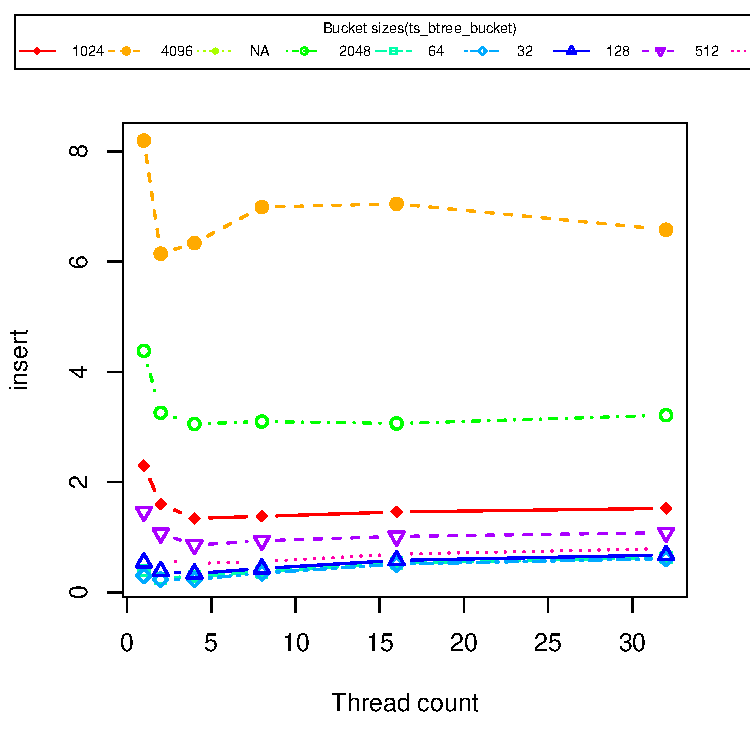
\includegraphics[width=1.0\textwidth]{plots/i7/plot_1_ts_btree_bucketinsert}
    }
    \subfloat[Search] {
        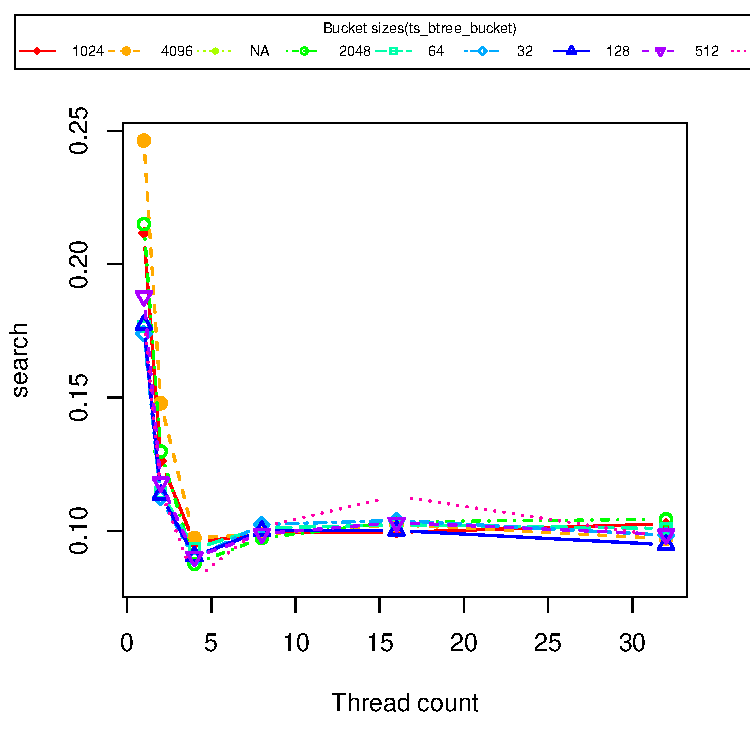
\includegraphics[width=1.0\textwidth]{plots/i7/plot_1_ts_btree_bucketsearch}
    }
    \label{fig:ts_i7_shake_btree}
    \caption{Multithreaded scaling of the binary tree bucket with varying sizes on the
    i7 machine (4 cores). Testing done with the shakespeare dataset.}
\end{figure}
\end{landscape}
